\section{Problem Description and Cache Structure}
\label{sec:Cache Structure}
\subsection{Notation and Problem Description}
The graph $G$ = ($V$, $E$) studied in this paper is undirected; $V = \{v_1, v_2,..., v_n\}$ is the set of nodes and $E=\{e_1,e_2,...,e_k\}$ is the set of edges.
The weight of an edge $e$ is denoted by $w_e$.
$P_{a,b}$ represents the shortest path between $v_a$ and $v_b$. If there exists more than one shortest paths between $v_a$ and $v_b$, $P_{a,b}$ represents one of them.
$Q_{a,b}$ represents a query of the shortest path between $v_a$ and $v_b$.
A cache is denoted by $\Omega$ and its capacity is $|\Omega|$. $\Psi$ refers to cached contents. The size of a cache and cached contents are measured by the number of nodes. It is clear that the size of $\Psi$ is always no larger than the cache capacity, i.e., $|\Psi|\leq |\Omega|$ all the time.

The problem is formally defined as follows: given an undirected graph $G$ and a query log $L$, the query log records the queries of shortest paths of $G$.
A cache $\Omega$ caches a part of shortest paths. Now the cache $\Omega$ has been fully loaded and the weight of a single edge $e$ in $G$ changes from $w_e$ to $w_e'$. Some paths in the cache may not be the shortest paths any more.
The objective of our problem is to refresh the content of cache $\Omega$ so that the hit ratio of future queries is as high as possible. The size of cache is assumed to be smaller than the size of shortest paths queried in $L$.


\subsection{Cache Structure}
In this paper, we design a cache structure to store and access paths in a cache.
In essence, the cache structure needs to satisfy two requirements: fast response and space efficiency.
We use a bitmap structure to index shortest paths. The bitmap structure was first developed for database use in the Model 204 product from Computer Corporation of America \citep{ONeil1997}. Now bitmap is commonly used in databases and data warehouses \citep{Wang2016}.

The cache structure proposed includes two parts of information: the path array that stores shortest paths and the bitmap that is used to index paths.
%The path array tells what nodes are contained in a certain path, while the bitmap tells which paths contain a certain node.
A bitmap is a 2-dimensional array.
The horizonal and vertical indices are paths and nodes, respectively.
If a path contains a certain node, the unit crossed by the path and node is marked with 1; otherwise, it is marked with 0.
The storage space of each unit only takes one bit. Here the name, bitmap.
The horizontal array indicated by a node $v_i$ is called a node vector $\vec{v_i}$.
Take Figure~\ref{fig:cache_structure} as an example. Three shortest paths $P_{0,5}$, $P_{2,4}$ and $P_{3,6}$ are stored in the form of arrays (Figure~\ref{fig:patharray}), and the bitmap of nodes is shown in Figure~\ref{fig:bitmap}.

\begin{figure*}[htbp]
\centering
   \subfigure[]
   {\label{fig:patharray}
   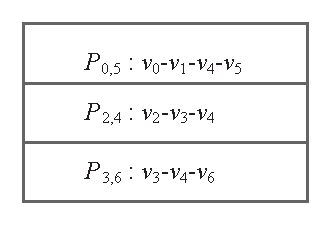
\includegraphics
   [height=3cm]{figure/Path_array.eps}}
   \subfigure[]
   {\label{fig:bitmap}
   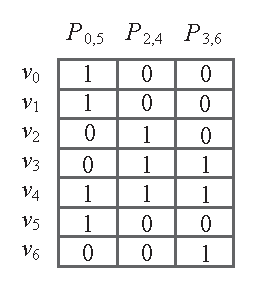
\includegraphics [height=3.5cm]{figure/bitmap.eps}}
 \caption{An example of cache structure.}
 \label{fig:cache_structure}
\end{figure*}



Given a query $Q_{s,e}$, we need to look up shortest paths that contain $v_s$ and $v_e$. The caching system looks up the bitmap and finds the node vectors $\vec{v_s}$ and $\vec{v_e}$. An AND operate is conducted to acquire $\vec{v_r}=\vec{v_s}$ AND $\vec{v_e}$. In $\vec{v_r}$, the bits whose value are 1 correspond to paths that contain $P_{s,e}$.

Now we analyze the space complexity of bitmap. For a graph with $N$ nodes, the maximum number of node-pair is $\frac{N*(N-1)}{2}$.
For any node-pair, at most one shortest path is loaded into the cache. Hence, the number of shortest paths in the cache is no larger than $\frac{N*(N-1)}{2}$. Moreover, the minimum size of a shortest path is 2, as a shortest path contains at least 2 nodes.
Therefore, a cache $\Omega$ can store at most $\min\{{\frac{|\Omega|}{2},\frac{N*(N-1)}{2}}\}$ shortest paths. Hence the number of columns in a bitmap is $\min\{{\frac{|\Omega|}{2},\frac{N*(N-1)}{2}}\}$. The most number of rows is the number of nodes $N$.
The number of bits needed in a bitmap is therefore $\min\{{\frac{|\Omega|}{2},\frac{N*(N-1)}{2}}\}*N$; and the number of bytes needed is $\lceil\frac{\min\{{\frac{|\Omega|}{2},\frac{N*(N-1)}{2}}\}*N}{8}\rceil$.
The space complexity of bitmap is $\mathcal O(\min\{{|\Omega|*N,N^3\}})$.


\section{Affected Shortest Path Detection}
\label{sec:detect-affected}
Before we refresh the cache, it is better for us to know which shortest paths are no longer shortest paths due to the change of an edge.
%By far, works on shortest paths storage structure \citep{bauer2009batch,d2013dynamically} have discussed how to detect affect paths with the change of graphs and update them.
%They generally store extra information to maintain the storage structure and update shortest paths.
%The problem of our paper is to refresh cache and reserving extra information for quick update of shortest paths seems digress.
%Moreover, in local servers, storage spaces are used to cache shortest paths as many as possible, leaving no spare space to store extra information for updating shortest paths.
%In this section, we propose simple methods to detect affected paths due to the change of an edge.

A shortest path $P_{i,j}=\langle v_i,...,v_j\rangle$ is \textbf{not affected} if the new shortest path $P'_{i,j}=\langle v_m,...,v_n\rangle$ due to the change of an edge $e$ is totally the same with $P_{i,j}$ in the node sequence.
Otherwise, $P_{i,j}$ is affected.
Hereafter, ``='' is used if two paths have the same sequence.
$e$ refers to the edge whose weight $w_e$ changes.
$P$ and $P'$ denote the shortest paths before and after $w_e$ changes, respectively.

It is noteworthy that even though $e$ is a part of $P_{i,j}$, if $P_{i,j}=P'_{i,j}$, $P_{i,j}$ is not affected. That is, the weight of a path has nothing to do with its being affected or not. The only thing that counts is the sequence.

Based on the definition of affected paths, we have the following corollaries.

\begin{corollary}
\label{corollary:weight-increase}
When $w_e$ increases, if $P_{i,j}$ is an affected path, then $P_{i,j}$ must contain $e$.
\end{corollary}

\begin{proof}
If $P_{i,j}$ does not contain $e$, then $P_{i,j}$ is still the shortest path when $w_e$ increases, that is, $P_{i,j}$ is not an affected path. Hence, if $P_{i,j}$ is an affected path, $P_{i,j}$ must contain $e$
\end{proof}

Compared to the increase of $w_e$, it is more difficult to detect affected paths when $w_e$ decreases, since paths that do not contain $e$ before $w_e$ decreases can also be affected paths.
The following corollary deals with the case that $w_e$ decreases.

\begin{corollary}
\label{corollary:weight-decrease}
When $w_e$ decreases, if $P_{i,j}$ is an affected path, then $P'_{i,j}$ must contain $e$.
\end{corollary}
\begin{proof}
Assume a shortest path $P_{i,j}$ is an affected path, and $P'_{i,j}$ does not contain edge $e$, then it has $P_{i,j}=P'_{i,j}$, indicating that $P_{i,j}$ is not an affected path. There is a conflict with the assumption. Therefore, $P'_{i,j}$ must contain edge $e$.
\end{proof}

\begin{corollary}
\label{thm:node-node}
The endpoints of $e$ are $v_a$ and $v_b$. $v_i$ and $v_j$ are two nodes where $v_j\neq v_a$, $v_j\neq v_b$. Suppose $P_{i,j}$ does not contain $e$ (if there exist more than one shortest paths between $v_i$ and $v_j$, we suppose that at least one shortest path does not contain $e$).
For any adjacent node $v_{adj}$ of $v_j$, if $P_{i,adj}$ is in the form of $P_{i,adj}=\langle v_i,...,v_j,v_{adj}\rangle$, $P_{i,adj}$ does not contain $e$ either.
\end{corollary}


\begin{proof}
Since $v_j\neq v_a$, $v_j\neq v_b$, no matter what $v_{adj}$ is, $\langle v_j,v_{adj} \rangle$ can not be $e$. In addition, sequence $\langle v_i,...,v_j\rangle$ must be $P_{i,j}$ which does not contain $e$. Thus, $P_{i,{adj}}$ does not contain $e$.
\end{proof}

Since $v_a$ and $v_b$ are symmetric, the following statement still stands: $v_i$ and $v_j$ are two nodes where $v_i\neq v_a$, $v_i\neq v_b$. Suppose at least one path of $P_{i,j}$ does not contain $e$.
For any adjacent node $v_{adj}$ of $v_i$, if $P_{{adj},j}$ is in the form of $P_{adj,j}=\langle v_{adj},v_i,...,v_j\rangle$, $P_{adj,j}$ does not contain $e$ either.
\subsection{Node Expansion Algorithm}
Since it is easy to check affected shortest paths when $w_e$ increases, in the following, we pay our attention on the algorithms of detecting affected paths when $w_e$ decreases.
We propose a node expansion algorithm (NEA) in this subsection.

For the affected shortest path detection problem, the key problem is to decide which paths are detected. The paths that contain $e$ should be detected while the paths that do not contain $e$ are not necessary to be detected.
The graph is our problem is undirected, therefore a path from $v_i$ to $v_j$ is just the path from $v_j$ to $v_i$. To avoid detecting a path two times, we artificially assign a direction for paths.
$C_s$ ($C_t$) is used to record start nodes (termination nodes) of to-be-detected paths.
Every time, one node $v_s$ from $C_s$ and one node $v_t$ from $C_t$ comprise a node-pair, and we detect whether its shortest path is affected. $C_s$ ($C_t$) is expanded by adding adjacent nodes of $v_s$ ($v_t$).

The pseudo code is illustrated in Algorithm~\ref{alg:calmin}.
The endpoints of $e$ are $v_a$ and $v_b$.
From the implementation perspective, both $C_s$ and $C_t$ are queues in a FIFO manner.
First, $C_s$ is initialized with the only start node $v_a$.
In the outer loop, start node $v_s$ is the first node popped from $C_s$.
If the new shortest path $P'_{s,b}$ contains $e$ (line~\ref{algo:1conte}), then adjacent nodes of $v_s$ are appended into $C_s$ unless they have been added into $C_s$ ever before. If $P'_{s,b}$ does not contain $e$, according to Corollary~\ref{thm:node-node}, the adjacent node $v_{adj}$ of $v_s$ are not necessarily put into $C_s$ since $P'_{{adj},b}$ does not contain $e$.
\begin{algorithm}[htbp]
{\small
    \caption{NEA}
    \label{alg:calmin}
    \KwIn{A graph $G(V,E)$, the edge $e$ which decreases its weight and its endpoints $v_a$ and $v_b$;}
    \KwOut{The set of affected paths $S_\textit{aff}$;}

   add $v_a$ to $C_s$\;
   \While{$C_s~is~not~empty$}{
        $ v_s \leftarrow$  pop the first element from $C_s$\;
        calculate $P'_{s,b}$\;
        \If{ $P'_{s,b}$ contains $e$}{\label{algo:1conte}
            \For{each adjacent node $v_{adj}$  of  $v_s$}{
                    \If{ $v_{adj}$ has not been added into $C_s$ }{
                        append $v_{adj}$ to $C_s$;
                    }
                }

        add $v_b$ to $C_t$\;
        \While{$C_t~is~not~empty$}
        {
            $ v_t \leftarrow$  pop the first element from $C_t$\;
            calculate $P'_{s,t}$\;
            \If{ $P'_{s,t}$ contains $e$}{
                %$Found \leftarrow true$\;
                \For{each adjacent node $v_{adj}$ of $v_t$}{
                    \If{$v_{adj}$ has not been added into $C_t$ }{
                        append $v_{adj}$ to $C_t$;
                    }
                }
                calculate $P_{s,t}$\;
                \If{$P_{s,t} \neq P'_{s,t}$}{\label{algo:1unequal}
                add $P_{s,t}$ to $S_\textit{aff}$;
                }
             }
             }
        }
   }

  \Return{$S_\textit{aff}$;}

}
\end{algorithm}

In the inner loop, $v_s$ is a fixed node.
$C_t$ is initialized with $v_b$.
$v_t$ is obtained by popping a node from $C_t$.
If $P'_{s,t}$ contains $e$, then adjacent nodes of $v_t$ are appended into $C_t$ unless they have been added into $C_t$ ever before.
For any path $P_{s,t}$, the algorithm checks whether $P_{s,t}=P'_{s,t}$, if not, $P_{s,t}$ is put into the set of affected paths $S_\textit{aff}$.


NEA satisfies both soundness and completeness. We first prove that the NEA is sound, i.e. any path in $S_\textit{aff}$ is an affected path. According to line~\ref{algo:1unequal} of the algorithm, if a path $P_{s,t}$ belongs to $S_\textit{aff}$, it has $P_{s,t} \neq P'_{s,t}$, so $P_{s,t}$ is an affected path.

Now we prove that NEA is complete. Assume that there exists an affected path $P_{s,t}$ that is not in $S_\textit{aff}$.
Based on Corollary~\ref{corollary:weight-decrease}, we know that $P'_{s,t}$ must contain the changed edge $e$. Hence, $v_s$ ($v_t$) is direct or indirectly connected with $v_a$ ($v_b$). According to NEA, $v_s$ ($v_t$) must have been added into $C_s$ ($C_t$).
Thus, $P_{s,t}$ must have been compared with $P'_{s,t}$.
Therefore, NEA can recognize $P_{s,t}$ as affected, and the assumption does not hold.
NEA is complete.

\begin{figure}[htbp]
\centering
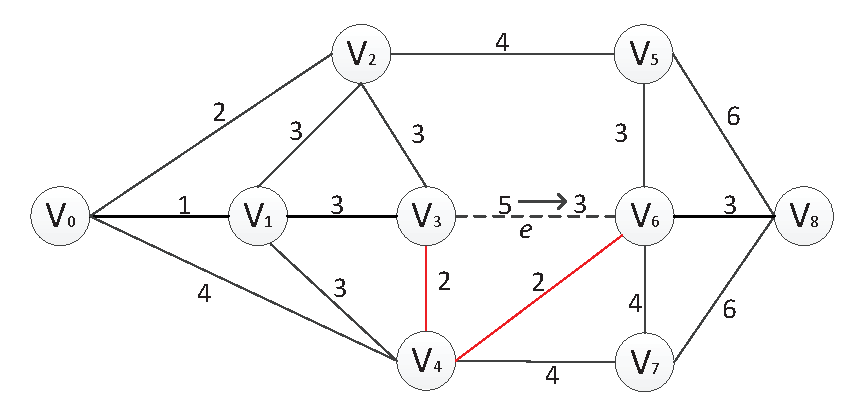
\includegraphics[scale=0.5]{figure/decrease.eps}
    \caption{An example of $w_e$ decreases.}
    \label{fig:decrease_example}
\end{figure}


Figure~\ref{fig:decrease_example} shows an example of computing affected paths when the weight of $e$ ($\langle v_3, v_6\rangle$) decreases from 5 to 3. Table~\ref{tab:algo1} shows the iteration process.

\begin{table}[htbp]
	\centering
	\caption{Iteration example of NEA.}
	\begin{tabular}{|l|l|l|l|l|l|}
    \hline
     & $C_s$ & $C_t$ & $v_s$ & $v_t$ & $S_\textit{aff}$ \\
    \hline
    $1$ & $\{v3\}$ 		  & $\emptyset$ 	  & null & null &  \\
    $2$ & $\emptyset$	  & $\emptyset$       & $v3$ & null &  \\
    $3$ & $\emptyset$  & $\{v6\}$          & $v3$ & null &  \\
	$4$ & $\{v1,v2,v4\}$  & $\emptyset$ 	  & $v3$ & $v6$ &  \\
    $5$ & $\{v1,v2,v4\}$  & $\{v4,v5,v7,v8\}$ & $v3$ & $v6$ & $P_{3,6}$ \\
    $6$ & $\{v1,v2,v4\}$  & $\{v5,v7,v8\}$    & $v3$ & $v4$ & $P_{3,6}$ \\
    $7$ & $\{v1,v2,v4\}$  & $\{v7,v8,v2\}$ 	  & $v3$ & $v5$ & $P_{3,6},P_{3,5}$ \\
    $8$ & $\{v1,v2,v4\}$  & $\{v8,v2\}$ 	  & $v3$ & $v7$ & $P_{3,6},P_{3,5}$ \\
    $9$ & $\{v1,v2,v4\}$ & $\{v2\}$ 		  & $v3$ & $v8$ & $P_{3,6},P_{3,5},P_{3,8}$ \\
    $10$ & $\{v1,v2,v4\}$ & $\emptyset$ 	  & $v3$ & $v2$ & $P_{3,6},P_{3,5},P_{3,8}$ \\
    $11$ & $\{v2,v4\}$ 	  & $\emptyset$ 	  & $v1$ & $v6$ & $P_{3,6},P_{3,5},P_{3,8}$ \\
    $12$ & $\{v4\}$		  & $\emptyset$ 	  & $v2$ & $v6$ & $P_{3,6},P_{3,5},P_{3,8}$ \\
    $13$ & $\{v4,v0,v5\}$		  & $\{v4,v5,v7,v8\}$ & $v2$ & $v6$ & $P_{3,6},P_{3,5},P_{3,8},P_{2,6}$ \\
    $14$ & $...$		  & $...$ 	  &... & ... & ... \\
    $15$ & $\{v4,v0,v5\}$    & $\emptyset$ 	  & $v2$ & $v8$ & $P_{3,6},P_{3,5},P_{3,8},P_{2,6},P_{2,8}$ \\
    $16$ & $\{v0,v5\}$ 	  & $\emptyset$ 	  & $v4$ & $v6$ & $P_{3,6},P_{3,5},P_{3,8},P_{2,6},P_{2,8}$  \\
    $17$ & $\{v5\}$ 	  & $\emptyset$ 	  & $v0$ & $v6$ & $P_{3,6},P_{3,5},P_{3,8},P_{2,6},P_{2,8}$  \\
    $18$ & $\emptyset$ 	  & $\emptyset$ 	  & $v5$ & $v6$ & $P_{3,6},P_{3,5},P_{3,8},P_{2,6},P_{2,8}$  \\
    \hline
    \end{tabular}
    \label{tab:algo1}
\end{table}

\iffalse
\begin{table}[htbp]
	\centering
	\caption{Iteration example of NEA.}
	\begin{tabular}{|l|l|l|l|l|l|}
    \hline
     & $C_s$ & $C_t$ & $v_s$ & $v_t$ & $S_\textit{aff}$ \\
    \hline
    $1$ & $\{v3\}$ 		  & $\emptyset$ 	  & null & null &  \\
    $2$ & $\emptyset$	  & $\emptyset$       & $v3$ & null &  \\
    $3$ & $\emptyset$  & $\{v6\}$          & $v3$ & null &  \\
	$4$ & $\{v1,v2,v4\}$  & $\emptyset$ 	  & $v3$ & $v6$ &  \\
    $5$ & $\{v1,v2,v4\}$  & $\{v4,v5,v7,v8\}$ & $v3$ & $v6$ & $P_{3,6}$ \\
    $6$ & $\{v1,v2,v4\}$  & $\{v5,v7,v8\}$    & $v3$ & $v4$ & $P_{3,6}$ \\
    $7$ & $\{v1,v2,v4\}$  & $\{v7,v8,v2\}$ 	  & $v3$ & $v5$ & $P_{3,6},P_{3,5}$ \\
    $8$ & $\{v1,v2,v4\}$  & $\{v8,v2\}$ 	  & $v3$ & $v7$ & $P_{3,6},P_{3,5}$ \\
    $9$ & $\{v1,v2,v4\}$ & $\{v2\}$ 		  & $v3$ & $v8$ & $P_{3,6},P_{3,5},P_{3,8}$ \\
    $10$ & $\{v1,v2,v4\}$ & $\emptyset$ 	  & $v3$ & $v2$ & $P_{3,6},P_{3,5},P_{3,8}$ \\
    $11$ & $\{v2,v4\}$ 	  & $\emptyset$ 	  & $v1$ & $v6$ & $P_{3,6},P_{3,5},P_{3,8}$ \\
    $12$ & $\{v4\}$		  & $\emptyset$ 	  & $v2$ & $v6$ & $P_{3,6},P_{3,5},P_{3,8}$ \\
    $13$ & $\{v4\}$		  & $\{v4,v5,v7,v8\}$ & $v2$ & $v6$ & $P_{3,6},P_{3,5},P_{3,8},P_{2,6}$ \\
    $14$ & $...$		  & $...$ 	  &... & ... & ... \\
    $15$ & $\{v4,v5\}$    & $\emptyset$ 	  & $v2$ & $v8$ & $P_{3,6},P_{3,5},P_{3,8},P_{2,6},P_{2,8}$ \\
    $16$ & $\{v5\}$ 	  & $\emptyset$ 	  & $v4$ & $v6$ & $P_{3,6},P_{3,5},P_{3,8}$ \\
    $17$ & $\emptyset$ 	  & $\emptyset$ 	  & $v5$ & $v6$ & $P_{3,6},P_{3,5},P_{3,8}$ \\
    \hline
    \end{tabular}
    \label{tab:algo1}
\end{table}
\fi

\subsection{Outward Node Expansion Algorithm}
\label{sec:optimaization approaches}

In the above subsection, we introduce a basic method NEA to compute affected shortest paths when the weight of a certain edge decreases.
The above algorithm mainly has two components: which paths are detected and how to check whether they are affected.
In this part, we will present how to improve determining which paths are detected.

For ease of illustration, we first introduce the concept of \textbf{node distance}. The node distance $d(i,j)$ between $v_i$ and $v_j$ represents the minimum number of nodes among all paths from $v_i$ to $v_j$. When weights of edges in a graph become all-1, $w(i,j)$ is equal to $d(i,j)$.
Let $S_d(v_a)$ be the set of nodes whose node distance from $a$ is $d$.
%If a sequence $S=\langle v_a,v_1,...,vi,..,vn\rangle$ satisfies that the $i$th element $v_i\in S_i(v_a)$, we say it is an orderly sequence since the order of elements comply with the order of node distances.

\begin{corollary}
\label{thm:reduce-end-node}
Suppose the endpoints of $e$ are $v_a$ and $v_b$, and $v_i$ is an arbitrary node. If for any node $v_j \in S_d(v_b)$, $P_{i,j}$ does not contain $e$, then for any node $v_{j+1}\in S_{d+1}(v_b)$, one of the following stands: $S=\langle v_i,...,v_j,v_{j+1}\rangle$ is a shortest path and it does not contain $e$; $S$ is not a shortest path.
\end{corollary}
\begin{proof}
For any node $v_{j+1}\in S_{d+1}(v_b)$, if $P_{i,j+1}=\langle v_i,...,v_j,v_{j+1}\rangle$, $v_j\in S_d(v_b)$, and $P_{i,j}$ does not contain $e$, then according to Corollary~\ref{thm:node-node}, $P_{i,j+1}$ does not contain $e$.
\end{proof}

Recall the algorithm NEA, although start nodes are added to $C_s$ in a FIFO order i.e., nodes are expanded in a breath-first manner, the nodes in $C_s$ are not discriminated based on the node distance from $v_a$.
In this subsection, we expand nodes based on their distances from $v_a$. Thus, the algorithm is called outward node expansion algorithm (ONE).
An auxiliary set $C'_s$ is employed to store the nodes that are expanded from the nodes in $C_s$, therefore, $C_s=S_{d}(v_a)$ while $C'_s=S_{d+1}(v_a)$.
The pseudo code of ONE is described in Algorithm~\ref{alg:candpath}.

\begin{algorithm}[htbp]
{\small
    \caption{{\textsc{ONE}} }
    \label{alg:candpath}
    \KwIn{A graph $G(V,E)$, the edge $e$ which decreases its weight and its endpoints $v_a$ and $v_b$;}
    \KwOut{The set of affected paths $S_\textit{aff}$;}
    add $v_b$ to $C_t$ and  $C'_t$\;\label{algo:2inis}
   \While{$C_t~is~not~empty$}
        {
            $ v_t \leftarrow$  pop the first element from $C_t$\;
            calculate $P'_{a,t}$\;
            \If{ $P'_{a,t}$ contains $e$}{
                %$Found \leftarrow true$\;
                \For{each adjacent node $v_{adj}$ of $v_t$}{
                     \If{$v_{adj}$ has not been added into $C_t$ }{
                         append $v_{adj}$ to $C_t$\;
                         append $v_{adj}$ to $C'_t$\;
                         }
                }
                calculate $P_{a,t}$\;
                \If{$P_{a,t} \neq P'_{a,t}$}{
                add $P_{a,t}$ to $S_\textit{aff}$;
                }
             }
        }\label{algo:2inie}
    replace $C_t$ with $C'_t$\;
    \For{each adjacent node $v_{adj}$  of  $v_a$}{
        add $v_{adj}$ to $C_s$\;
    }
    \While{$C_s$ is not empty}{
     $C'_s \leftarrow \emptyset$;$C'_t \leftarrow \emptyset$; \tcp{initialize auxiliary sets}

     %$C_e \leftarrow \emptyset$\;
     \For{ each node $v_s$ in $C_s$}{
           calculate $P'_{s,b}$\;
        \If{ $P'_{s,b}$ contains $e$}{\label{algo:2conte}
            \For{each adjacent node $v_{adj}$  of  $v_s$}{
                    \If{ $v_{adj}$ has not been added into $C_s$ }{
                        add $v_{adj}$ to $C'_s$; \tcp{store $v_{adj}$ for the next round}
                    }
                }

     \For{ each $v_t$ in ${C_t}$}{\label{algo:2forvt}
            calculate $P'_{s,t}$\;
            \If{ $P'_{s,t}$ contains $e$}{

                add $v_t$ to $ C'_t$; \tcp{store $v_t$ for the next round}
                calculate $P_{s,t}$\;\label{algo:2calPse}
                \If{$P_{s,t} \neq P'_{s,t}$}{\label{algo:2unequal}
                add $P_{s,t}$ to $S_\textit{aff}$\;\label{algo:2end}
                }
             }
     }
     }
 }
   replace $C_s$ and  $C_t$  with $C'_s $ and $C'_t$, respectivley\;
}
}
  \Return{$S_\textit{aff}$}
\end{algorithm}

For fixed $v_a$, if a node $v_t$ satisfies that (1) $v_t$ is connected with $v_b$; and (2) $P'_{a,t}$ contains $e$, we add $v_t$ into $C_t$ (line~\ref{algo:2inis}-\ref{algo:2inie}).
Starting from iteration $d=0$, we try to reduce the size of $C_t$.
For a node $v_t\in C_t$, if $P'_{s,t}$ does not contain $e$ for any node $v_s\in S_{d}(v_a)$, then according to Corollary~\ref{thm:reduce-end-node}, $P'_{s,t}$ does not contain $e$ for any node $v_s\in S_{d+1}(v_a)$.
Therefore, $v_t$ is deleted from $C_t$, reflecting by not adding into $C'_t$.
Hence, ONE saves the time of visiting $v_t$ in the $d+1$th (and latter iterations) and calculating corresponding shortest paths.

Based on ONE, the iteration process of example Figure~\ref{fig:decrease_example} is displayed in Table~\ref{tab:algo2}.
\begin{table}[htbp]
	\centering
	\caption{Iteration example of ONE.}
	\begin{tabular}{|l|l|l|l|l|l|}
    \hline
     & $C_s$ & $C_t$ & $v_s$ & $v_t$ & $S_\textit{aff}$ \\
    \hline
    $1$ & $\{v3\}$ 		  & $\emptyset$ 	  & null & null &  \\
    $2$ & $\emptyset$	  & $\emptyset$       & $v3$ & null &  \\
    $3$ & $\emptyset$  & $\{v6\}$          & $v3$ & null &  \\
	$4$ & $\{v1,v2,v4\}$  & $\emptyset$ 	  & $v3$ & $v6$ &  \\
    $5$ & $\{v1,v2,v4\}$  & $\{v4,v5,v7,v8\}$ & $v3$ & $v6$ & $P_{3,6}$ \\
    $6$ & $\{v1,v2,v4\}$  & $\{v5,v7,v8\}$    & $v3$ & $v4$ & $P_{3,6}$ \\
    $7$ & $\{v1,v2,v4\}$  & $\{v2,v7,v8\}$ 	  & $v3$ & $v5$ & $P_{3,6},P_{3,5}$ \\
    $8$ & $\{v1,v2,v4\}$  & $\{v7,v8\}$ 	  & $v3$ & $v2$ & $P_{3,6},P_{3,5}$ \\
    $9$ & $\{v1,v2,v4\}$ & $\{v8\}$ 		  & $v3$ & $v7$ & $P_{3,6},P_{3,5}$ \\
    $10$ & $\{v1,v2,v4\}$ & $\emptyset$ 	  & $v3$ & $v8$ & $P_{3,6},P_{3,5},P_{3,8}$ \\
    $11$ & $\{v2,v4\}$ 	  & $\emptyset$ 	  & $v1$ & $v6$ & $P_{3,6},P_{3,5},P_{3,8}$ \\
    $12$ & $\{v4\}$		  & $\{v6,v5,v8\}$ 	  & $v2$ & $null$ & $P_{3,6},P_{3,5},P_{3,8}$ \\
    $13$ & $\{v4,v0,v5\}$		  & $\{v5,v8\}$ 	      & $v2$ & $v6$ & $P_{3,6},P_{3,5},P_{3,8},P_{2,6}$ \\
    $14$ & $\{v4,v0,v5\}$		  & $\{v8\}$ 	      & $v2$ & $v5$ & $P_{3,6},P_{3,5},P_{3,8},P_{2,6}$ \\
    $15$ & $\{v4,v0,v5\}$		  & $\emptyset$ 	  & $v2$ & $v8$ & $P_{3,6},P_{3,5},P_{3,8},P_{2,6},P_{2,8}$ \\
    $16$ & $\{v0,v5\}$ 	  & $\emptyset$ 	  & $v4$ & $v6$ & $P_{3,6},P_{3,5},P_{3,8},P_{2,6},P_{2,8}$\\
    $17$ & $\{v5\}$ 	  & $\emptyset$ 	  & $v0$ & $v6$ & $P_{3,6},P_{3,5},P_{3,8},P_{2,6},P_{2,8}$\\
    $18$ & $\emptyset$ 	  & $\emptyset$ 	  & $v5$ & $v6$ & $P_{3,6},P_{3,5},P_{3,8},P_{2,6},P_{2,8}$ \\
    \hline
    \end{tabular}
    \label{tab:algo2}
\end{table}

\iffalse
\begin{table}[htbp]
	\centering
	\caption{Iteration example of ONE.}
	\begin{tabular}{|l|l|l|l|l|l|}
    \hline
     & $C_s$ & $C_t$ & $v_s$ & $v_t$ & $S_\textit{aff}$ \\
    \hline
    $1$ & $\{v3\}$ 		  & $\emptyset$ 	  & null & null &  \\
    $2$ & $\emptyset$	  & $\emptyset$       & $v3$ & null &  \\
    $3$ & $\emptyset$  & $\{v6\}$          & $v3$ & null &  \\
	$4$ & $\{v1,v2,v4\}$  & $\emptyset$ 	  & $v3$ & $v6$ &  \\
    $5$ & $\{v1,v2,v4\}$  & $\{v4,v5,v7,v8\}$ & $v3$ & $v6$ & $P_{3,6}$ \\
    $6$ & $\{v1,v2,v4\}$  & $\{v5,v7,v8\}$    & $v3$ & $v4$ & $P_{3,6}$ \\
    $7$ & $\{v1,v2,v4\}$  & $\{v2,v7,v8\}$ 	  & $v3$ & $v5$ & $P_{3,6},P_{3,5}$ \\
    $8$ & $\{v1,v2,v4\}$  & $\{v7,v8\}$ 	  & $v3$ & $v2$ & $P_{3,6},P_{3,5}$ \\
    $9$ & $\{v1,v2,v4\}$ & $\{v8\}$ 		  & $v3$ & $v7$ & $P_{3,6},P_{3,5}$ \\
    $10$ & $\{v1,v2,v4\}$ & $\emptyset$ 	  & $v3$ & $v8$ & $P_{3,6},P_{3,5},P_{3,8}$ \\
    $11$ & $\{v2,v4\}$ 	  & $\emptyset$ 	  & $v1$ & $v6$ & $P_{3,6},P_{3,5},P_{3,8}$ \\
    $12$ & $\{v4\}$		  & $\{v6,v8\}$ 	  & $v2$ & $null$ & $P_{3,6},P_{3,5},P_{3,8}$ \\
    $13$ & $\{v4\}$		  & $\{v8\}$ 	      & $v2$ & $v6$ & $P_{3,6},P_{3,5},P_{3,8},P_{2,6}$ \\
    $14$ & $\{v4\}$		  & $\emptyset$ 	  & $v2$ & $v8$ & $P_{3,6},P_{3,5},P_{3,8},P_{2,6},P_{2,8}$ \\
    $15$ & $\{v5\}$ 	  & $\emptyset$ 	  & $v4$ & $v6$ & $P_{3,6},P_{3,5},P_{3,8}$ \\
    $16$ & $\emptyset$ 	  & $\emptyset$ 	  & $v5$ & $v6$ & $P_{3,6},P_{3,5},P_{3,8}$ \\
    \hline
    \end{tabular}
    \label{tab:algo2}
\end{table}
\fi


\subsection{Inward Node Expansion Algorithm}

In this section, we present another two techniques to improve the efficiency of affected shortest path detection. We still focus on the order to generate node-pairs with each from $C_s$ and $C_t$, respectively.

\begin{corollary}
\label{thm:longer}
Suppose $v_a$ and $v_b$ are endpoints of $e$, $v_s$ ($v_t$) is a node connected with $v_a$ ($v_b$). If $P_{s,t}$ contains $e$, then $P_{s,t}$ must have the form $\langle v_s,...,v_a,v_b,...,v_k,...,v_t\rangle $ and at least one path of $P_{s,k}$ contains $e$.
\end{corollary}

\begin{proof}
Since $P_{s,t}$ is a shortest path, its subpath $\langle v_s,...,v_a,v_b,...,v_k\rangle $ is also a shortest path, i.e., $P_{s,k}=\langle v_s,...,v_a,v_b,...,v_k\rangle$ and $P_{s,k}$ contains $e$.
\end{proof}

Corollary~\ref{thm:longer} tells us that for a node $v_s$ connected with $v_a$, if we have detected a path $P_{s,t}$ where $v_t\in S_{d}(v_b)$, then the nodes $v_k$ on $P'_{s,t}=\langle v_s,...v_b,...,v_k,...v_t\rangle$ are not necessarily visited. If only $P'_{s,t}$ contains $e$, $P'_{s,k}$ contains $e$ as well.

Next we consider how to optimize the process to check whether a shortest path is affected.
\begin{corollary}
\label{thm:check}
Suppose the end nodes of $e$ are $v_a$ and $v_b$. When $w_e$ decreases, if $P_{a,b}$ is an affected path, then any shortest path $P'_{s,e}$ which contains $e$ is an affected path, i.e., $P'_{s,e} \neq P_{s,e}$.
\end{corollary}


\begin{proof}
Assume there exists a path $P'_{s,e}$ which contains $e$ and $P_{s,e}=P'_{s,e}$.
As $P_{a,b}$ is an affected shortest path, we know $P_{a,b}=S1=\langle v_a,v_m,...,v_n,v_b\rangle$ and $P'_{a,b}=S2=\langle v_a,v_b\rangle=e$ and $w'_{S2}<w_{S1}=w'_{S1}<w_{S2}$.
Since $P'_{s,e}$ contains $e$, the sequence of $P'_{s,e}$ must be $S3=\langle v_s,...,v_a,v_b,...,v_e\rangle $. If we substitute $\langle v_a,v_b\rangle$ ($S2$) in $S3$ with $S1$, we have $S4=\langle v_s,...,v_a,v_m,...,v_n,v_b,...,v_e\rangle$. It is clearly that $w_{S4}<w_{S3}$, therefore $P_{s,e}$ can not be $S3$. The assumption does not hold; therefore our corollary stands.
\end{proof}

According to Corollary~\ref{thm:check}, the process of detecting whether a path is affected is shortened. If $P_{a,b}$ is an affected shortest path, we can avoid the calculation of $P_{s,e}$ in line~\ref{algo:2calPse} and comparison with $P'_{a,b}$ in line~\ref{algo:2unequal} of Algorithm~\ref{alg:candpath}, since $P'_{s,e}$ contains $e$ (line~\ref{algo:2conte} of Algorithm~\ref{alg:candpath}), so we can know $P_{s,e}$ is an affected path directly.

We have another optimized algorithm inward node expansion algorithm (INE). The term ``inward'' is because nodes of $C_t$ are visited from ones far way to $v_b$.
Since the main logic of INE is the same with ONE, we only demonstrate the different lines. INE is to replace line~\ref{algo:2forvt}-\ref{algo:2end} of ONE with the code in Algorithm~\ref{alg:candpathplus}.



\begin{algorithm}[htbp]
{\small
     \caption{{\textsc{INE}} }
    \label{alg:candpathplus}
      \While{$C_t$ is not empty}{
          $v_t  \leftarrow $ pop the node in $C_t$ which has the largest node distance from $v_b$\;
          calculate $P'_{s,t}$\;
          \If{ $P'_{s,t}$ contains $e$}{
                \For{ each $v_k$ lies on path $P'_{s,t}$}{
                   add $v_k$ into $C'_t$\; \label{algo:3add}
                   pop $v_k$ from ${C_t}$\;\label{algo:3pop}
                \If{ $P_{a,b}$ is an affected path}
                {\label{algo:3ifpab}
                     add $P_{s,k}$ to $S_\textit{aff}$\;
                }
                \Else{
                    calculate  $P_{s,k}$\;
                   \tcp{$P'_{s,k}$ is the subpath of $P'_{s,t}$}
                    \If{$P_{s,t} \neq P'_{s,t}$}{
                    add $P_{s,t}$ to $S_\textit{aff}$\;
                    }
               }

          }
        }
     }
}
\end{algorithm}

In Algorithm~\ref{alg:candpathplus}, line~\ref{algo:3add}-\ref{algo:3pop} indicate that if $v_k$ is on a shortest path which contains $e$, then $v_k$ is added into $C'_t$ for the next iteration directly even though it has not been visited in this round of iteration. The IF sentence in line~\ref{algo:3ifpab} takes the advantage of Corollary~\ref{thm:check}.



Take Figure~\ref{fig:decrease_example} as an example, the iteration process by INE is illustrated in Table~\ref{tab:algo3}.
\begin{table}[htbp]
	\centering
	\caption{Iteration example of INE.}
	\begin{tabular}{|l|l|l|l|l|l|}
    \hline
     & $C_s$ & $C_t$ & $v_s$ & $v_t$ & $S_\textit{aff}$ \\
    \hline
    $1$ & $\{v3\}$ 		  & $\emptyset$ 	  & null & null &  \\
    $2$ & $\emptyset$	  & $\emptyset$       & $v3$ & null &  \\
    $3$ & $\emptyset$  & $\{v6\}$          & $v3$ & null &  \\
	$4$ & $\{v1,v2,v4\}$  & $\emptyset$ 	  & $v3$ & $v6$ &  \\
    $5$ & $\{v1,v2,v4\}$  & $\{v4,v5,v7,v8\}$ & $v3$ & $v6$ & $P_{3,6}$ \\
    $6$ & $\{v1,v2,v4\}$  & $\{v5,v7,v8\}$    & $v3$ & $v4$ & $P_{3,6}$ \\
    $7$ & $\{v1,v2,v4\}$  & $\{v2,v7,v8\}$ 	  & $v3$ & $v5$ & $P_{3,6},P_{3,5}$ \\
    $8$ & $\{v1,v2,v4\}$  & $\{v7,v8\}$ 	  & $v3$ & $v2$ & $P_{3,6},P_{3,5}$ \\
    $9$ & $\{v1,v2,v4\}$ & $\{v8\}$ 		  & $v3$ & $v7$ & $P_{3,6},P_{3,5}$ \\
    $10$ & $\{v1,v2,v4\}$ & $\emptyset$ 	  & $v3$ & $v8$ & $P_{3,6},P_{3,5},P_{3,8}$ \\
    $11$ & $\{v2,v4\}$ 	  & $\emptyset$ 	  & $v1$ & $v6$ & $P_{3,6},P_{3,5},P_{3,8}$ \\
    $12$ & $\{v4\}$		  & $\{v6,v5,v8\}$ 	      & $v2$ & $null$ & $P_{3,6},P_{3,5},P_{3,8}$ \\
    $13$ & $\{v4\}$		  & $\{v5\}$ 	  & $v2$ & $v8$ & $P_{3,6},P_{3,5},P_{3,8},P_{2,6},P_{2,8}$ \\
    $14$ & $\{v4,v0,v5\}$		  & $\emptyset$ 	  & $v2$ & $v5$ & $P_{3,6},P_{3,5},P_{3,8},P_{2,6},P_{2,8}$ \\
    $15$ & $\{v0,v5\}$ 	  & $\emptyset$ 	  & $v4$ & $v6$ & $P_{3,6},P_{3,5},P_{3,8},P_{2,6},P_{2,8}$  \\
     $16$ & $\{v5\}$ 	  & $\emptyset$ 	  & $v0$ & $v6$ & $P_{3,6},P_{3,5},P_{3,8},P_{2,6},P_{2,8}$  \\
    $17$ & $\emptyset$ 	  & $\emptyset$ 	  & $v5$ & $v6$ & $P_{3,6},P_{3,5},P_{3,8},P_{2,6},P_{2,8}$  \\
    \hline
    \end{tabular}
    \label{tab:algo3}
\end{table}

\iffalse
\begin{table}[htbp]
	\centering
	\caption{Iteration example of INE.}
	\begin{tabular}{|l|l|l|l|l|l|}
    \hline
     & $C_s$ & $C_t$ & $v_s$ & $v_t$ & $S_\textit{aff}$ \\
    \hline
    $1$ & $\{v3\}$ 		  & $\emptyset$ 	  & null & null &  \\
    $2$ & $\emptyset$	  & $\emptyset$       & $v3$ & null &  \\
    $3$ & $\emptyset$  & $\{v6\}$          & $v3$ & null &  \\
	$4$ & $\{v1,v2,v4\}$  & $\emptyset$ 	  & $v3$ & $v6$ &  \\
    $5$ & $\{v1,v2,v4\}$  & $\{v4,v5,v7,v8\}$ & $v3$ & $v6$ & $P_{3,6}$ \\
    $6$ & $\{v1,v2,v4\}$  & $\{v5,v7,v8\}$    & $v3$ & $v4$ & $P_{3,6}$ \\
    $7$ & $\{v1,v2,v4\}$  & $\{v2,v7,v8\}$ 	  & $v3$ & $v5$ & $P_{3,6},P_{3,5}$ \\
    $8$ & $\{v1,v2,v4\}$  & $\{v7,v8\}$ 	  & $v3$ & $v2$ & $P_{3,6},P_{3,5}$ \\
    $9$ & $\{v1,v2,v4\}$ & $\{v8\}$ 		  & $v3$ & $v7$ & $P_{3,6},P_{3,5}$ \\
    $10$ & $\{v1,v2,v4\}$ & $\emptyset$ 	  & $v3$ & $v8$ & $P_{3,6},P_{3,5},P_{3,8}$ \\
    $11$ & $\{v2,v4\}$ 	  & $\emptyset$ 	  & $v1$ & $v6$ & $P_{3,6},P_{3,5},P_{3,8}$ \\
    $12$ & $\{v4\}$		  & $\{v8\}$ 	      & $v2$ & $null$ & $P_{3,6},P_{3,5},P_{3,8}$ \\
    $13$ & $\{v4\}$		  & $\emptyset$ 	  & $v2$ & $v8$ & $P_{3,6},P_{3,5},P_{3,8},P_{2,6},P_{2,8}$ \\
    $14$ & $\{v5\}$ 	  & $\emptyset$ 	  & $v4$ & $v6$ & $P_{3,6},P_{3,5},P_{3,8}$ \\
    $15$ & $\emptyset$ 	  & $\emptyset$ 	  & $v5$ & $v6$ & $P_{3,6},P_{3,5},P_{3,8}$ \\
    \hline
    \end{tabular}
    \label{tab:algo3}
\end{table}
\fi

Now we compare the performance of three algorithms. The nodes visited by the three proposed algorithms are displayed in Table~\ref{tab:algocomp}.
The numbers of nodes visited are NEA$>$ONE$>$INE, and the numbers of iterations for the three methods are still NEA$>$ONE$>$INE.
\begin{table}[htbp]
	\centering
	\caption{Performance comparison of algorithms.}
	\begin{tabular}{|l|l|l|l|l|}
    \hline
     & $v_s$ & $C_t$ (NEA) & $C_t$ (ONE) & $C_t$ (INE)  \\
    \hline
    $1$ & $v3$   & $\{v2,v4,v5,v6,v7,v8\}$	  & $\{v2,v4,v5,v6,v7,v8\}$	& $\{v2,v4,v5,v6,v7,v8\}$	 \\
    $2$ & $v1$   & $\{v6\}$	 &  $\{v6\}$	&  $\{v6\}$ \\
     $3$ & $v2$   & $\{v4,v5,v6,v7,v8\}$	 & $\{v5,v6,v8\}$& $\{v5,v8\}$	 \\
     $4$ & $v4$   & $\{v6\}$	 & $\{v6\}$	& $\{v6\}$	 \\
      $5$ & $v0$   & $\{v6\}$	 & $\{v6\}$	& $\{v6\}$ \\
     $6$ & $v5$   & $\{v6\}$	 & $\{v6\}$	& $\{v6\}$ \\
    \hline
    \end{tabular}
    \label{tab:algocomp}
\end{table}
\iffalse
\begin{table}[htbp]
	\centering
	\caption{Performance comparison of algorithms.}
	\begin{tabular}{|l|l|l|l|l|}
    \hline
     & $v_s$ & $C_t$(NEA) & $C_t$(ONE) & $C_t$(INE)  \\
    \hline
    $1$ & $v3$   & $\{v2,v4,v5,v6,v7,v8\}$	  & $\{v2,v4,v5,v6,v7,v8\}$	& $\{v2,v4,v5,v6,v7,v8\}$	 \\
    $2$ & $v1$   & $\{v6\}$	 &  $\{v6\}$	&  $\{v6\}$ \\
     $3$ & $v2$   & $\{v4,v5,v6,v7,v8\}$	 & $\{v6,v8\}$& $\{v8\}$	 \\
     $3$ & $v4$   & $\{v6\}$	 & $\{v6\}$	& $\{v6\}$	 \\
     $3$ & $v5$   & $\{v6\}$	 & $\emptyset$	& $\emptyset$ \\
    \hline
    \end{tabular}
    \label{tab:algocomp}
\end{table}
\fi

\modify{
In terms of the time complexity, NEA computes nodes that are connected with start and end nodes, composing start and end sets. For a graph with $N$ nodes, the time complexity is $\mathcal O(N^2)$.
ONE and INE are improvements of NEA. In the worst case, the start and end sets still include all nodes. Thus, the time complexity of two optimized algorithms are still $\mathcal O(N^2)$.
}


